%Mark says: This should describe the aims of your research study and why the research problem is important. It should also set the scene for everything that follows.

%Lucie says: 
%*Fact check my %mythology, %science-history and %modern-day-view paragraphs.
%*Fusion
%*Structure
%*Energy transport from core to photosphere
%*Atmosphere (show classic T, rho plot)
%*Magnetic field (permeates entire Sun ands atmosphere)
%   *a couple of statements about internal dynamo
%   *field transported by ("frozen-in") bouyant plasma in the convection zone (flux tubes created by dynamo)
%   *Sunspots to coronal loops
%*Magnetic activity
%   *reconnection
%   *cme
%   *flares   
%*Sunquakes
%*My science question


%angstrom Å


\section{Introduction}
%Chronological soft intro; use some of the lit review,
%making sure to emphasize the connection to solar flares;Look at early papers predicting sunquakes(Wolff 70s and Kosovichev and Zharkova);the importance of sunquakes
During this age of space-born solar astronomy, understanding the highly dynamic environment of the Sun's atmosphere is a study enriched by a wealth of high detail observations. With each newly launched space instrument the spatial resolution of collected data increases, which coupled with those spacecraft that are tailored to capture light of previously unobserved wavelengths, often leads to new phenomena being observed. Eruptive solar flares fall into this category, in that spacecraft have provided observations that challenge the current theoretical view that the standard eruptive flare model (CSHKP model: \citep{1964NASSP..50..451C, 1966Natur.211..695S, 1974SoPh...34..323H, 1976SoPh...50...85K} puts forward.

Solar flares are one of the most energetic events to occur in the Sun's atmosphere, where by stored magnetic energy is released in the form of heat, mass motions, and accelerated particles. This highly dynamic process produces many measurable emission signatures at wavelengths from $\gamma$-rays to radio waves. Many of these observed signatures agree with the CSHKP model, however, this is not the full picture. The standard flare model has been modified to include new observations many times over the years (e.g., \cite{2011LRSP....8....6S}) and is still unable to describe some observed phenomena. 

Sunquakes are an observable feature during some solar flares that the standard model is unable to explain. It is believed that they are the result of energy and momentum released during the flare impacting the lower solar atmosphere. If a sufficient amount of momentum is imparted on the lowest atmospheric layer, then acoustic waves or 'sunquakes' are produced. The challenges presented in studying this phenomena are mainly associated with the ambiguous nature of the mechanism by which sunquakes are generated. Many ideas for the sunquakes progenitors have been put forward but at this point in time observable signatures do not always show a clear cut evidence aligning with current theories. Therefore this is an exciting time to be investigating the formation mechanisms of sunquakes and could also contribute to our overall understanding of solar flares.      
%%%%%%%%%%%%%%%%%%%%%%%%%%%%%%%%%%%%%%%%%%%%%%%%
%%%%%%%%END OF SOFT INTRO%%%%%%%%%%%%%%%%%%%%%%%
\subsection{Solar Atmosphere}
The solar atmosphere can be described as having four components, the corona, transition region, chromosphere and photosphere, see Figure \ref{solatmpics}.

\begin{figure}[H]%\label{sunquake-cartoon}
  \begin{center}
  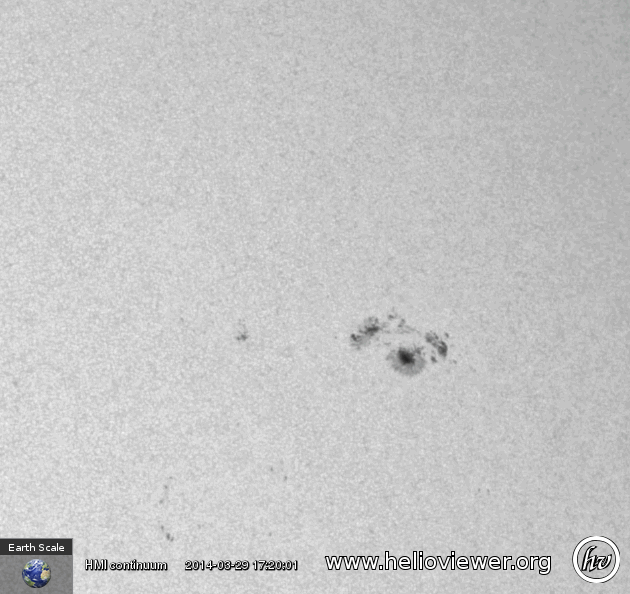
\includegraphics[width=0.20\textwidth]{2014_03_29_17_19_42_HMI_Int}%photsphere
  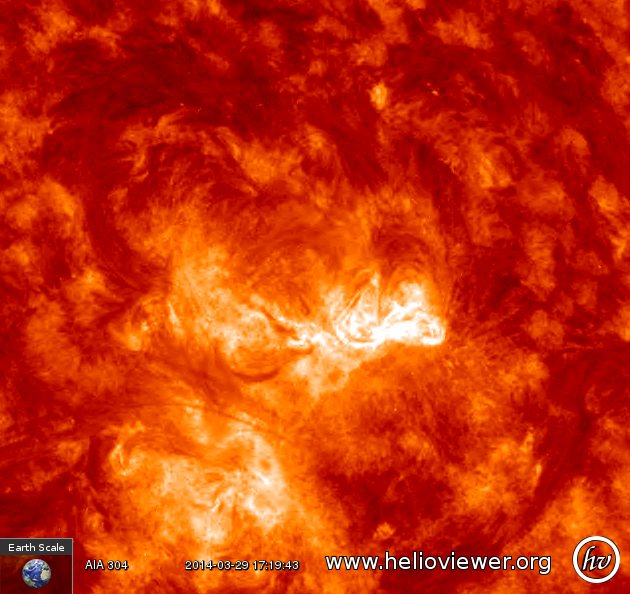
\includegraphics[width=0.20\textwidth]{2014_03_29_17_19_42_AIA_304}%chromosphere
  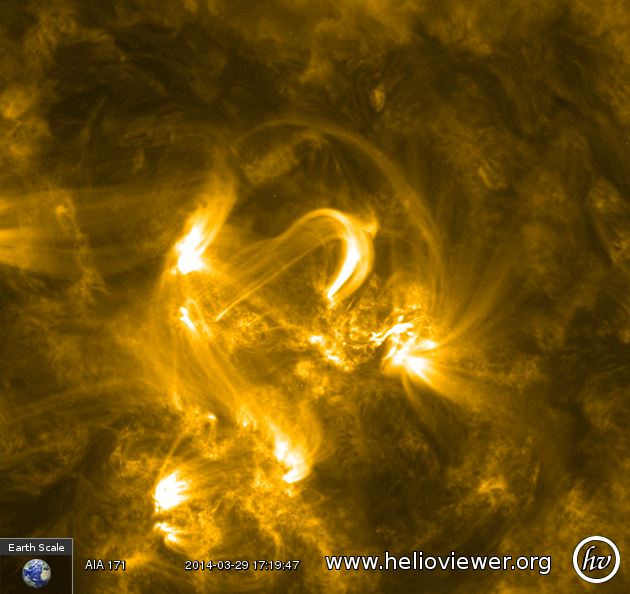
\includegraphics[width=0.20\textwidth]{2014_03_29_17_19_42_AIA_171}%tr
  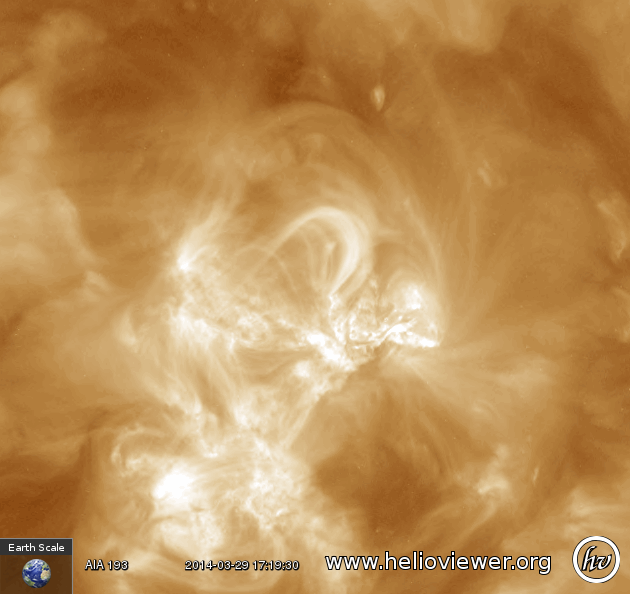
\includegraphics[width=0.20\textwidth]{2014_03_29_17_19_42_AIA_193}%corona
  \caption{ Images taken from the Solar Dynamics Observatory (SDO) instruments, the Helioseismic Magnetic Imager(HMI) and the Atmospheric Imaging Assembly (AIA) displaying the four main components of the solar atmosphere. From left to right layers of the solar atmosphere are increasing in altitude and temperature from the photosphere (SDO/HMI 6173 \AA\ continuum), to the chromosphere (SDO/AIA 304 \AA) through the transition region (SDO/AIA 171 \AA) then up to the corona (SDO/AIA 193 \AA). Images courtesy of \href{www.helioviewer.org}{www.helioviewer.org}}\label{solatmpics}
\end{center}
\end{figure}


For a sunquake to occur, energy released during a solar flare has to traverse these four layers propagating through many pressure scale heights as it does so. Pressure scale height is a measure of the distance over which pressure drops off by a factor of \emph{e}. For example, in the photosphere, $H\sim150$km, whereas in the corona, $H\sim100$Mm. Figure \ref{solar-atm-plot} shows how the solar atmosphere changes with height, temperature and density, for each of the atmospheric layers. Information in this section is taken from text books: \cite{2003dysu.book.....D, 2004soas.book.....F}


\subsubsection{The Photosphere}
The photosphere is the lowest in altitude of the atmospheric layers, forming a shell around the Sun with a radius somewhere between $\sim10$ - $10^{2}$ km. With an effective temperature of $T\sim5800$K, the photosphere decreases in temperature with radial distance to $\sim4400$K in the temperature minimum region. Emission from this part of the atmosphere is predominantly in the visible range. Contained in the photosphere, are neutral hydrogen atoms, ions and electrons. When a neutral hydrogen atom captures a free electron it forms H$^{-}$ ions, which via absorption of UV and infrared radiation increases the opacity of the region. Even though it is thought that electron capture is a rare occurrence, the population of H$^{-}$ ions is large enough to count for the majority of the photospheric opacity. The densest atmospheric layer, plasma pressure in the photosphere is dominant over magnetic pressure such that the plasma-beta, $\beta = p_{gas}/p_{mag} >> 1$. Because of frozen-in theorem (see section \ref{}) photospheric plasma dictates the motions of and to some extent, the morphology of the local magnetic field.

Granules are observed over almost the entire photosphere and are the physical representation of convection currents. Seen as the bright central part of the granule, buoyant, heated plasma rises from a region known as the convective zone, underneath the photosphere. As the material cools, it loses it's buoyancy and falls back toward the interior forming the darker areas surrounding the granule known as intergranular lanes.

Active regions on the photosphere contain sunspots, which are regions of intense magnetic field playing host to footpoints of loops that can extend out into interplanetary space. An active region is formed of at least two sunspots of opposing polarity. 
A sunspot is an approximately circular feature, made up of two main parts, the dark central umbra which is surrounded by the slightly lighter penumbra. The umbra hosts magnetic field lines that are tightly packed and pointing radially away from the Sun, whereas the penumbral magnetic field is more horizontal with respect to the solar surface. With a field strength of $\sim 10^{-1}$ Tesla, sunspots are regions in the photosphere where the magnetic pressure is dominant over plasma pressure, such that $\beta << 1$. Meaning that in these regions convection currents and radiative transfer are inhibited, with the latter being the idea behind a sunspot's dark appearance. \\



\begin{figure}[H]
  \begin{center}
    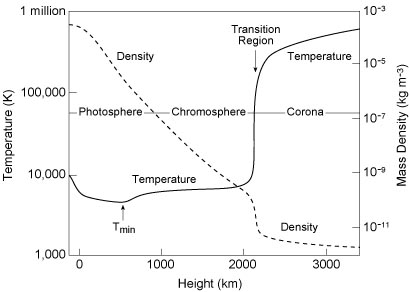
\includegraphics[width=0.6\textwidth]{solar-atm-plot}
\caption{The temperature of the solar atmosphere decreases from values near 6,000 degrees Kelvin at the visible photosphere to a minimum value of roughly 4,400 degrees Kelvin about 500 kilometres higher up. The temperature increases with height, slowly at first, then extremely rapidly in the narrow transition region, less than 100 kilometres thick, between the chromosphere and corona, from about $10^{4}$K to about $10^{6}$K. (Courtesy of Eugene Avrett, Smithsonian Astrophysical Observatory.)}\label{solatm}
  \end{center}
\end{figure}

\subsubsection{Chromosphere}
The next region of the atmosphere is the chromosphere which is situated above the photosphere. This layer of plasma is a few thousand kilometres (2000 - 3000 km) thick and is optically thin to visible light so is difficult to observe against the brightness of the photosphere. The temperature in this layer increases with height from 4400 K at the temperature minimum region to $\sim10^{5}$K near the transition region. As a result, plasma density decreases and $\beta$ drops, crossing unity near the transition region between the upper-chromosphere and corona. This means that the pressure scale height in this region is changing with altitude as a transition from the plasma to magnetic domain occurs. The chromosphere is observable in the optically thick H$\alpha$ line in a red wavelength due to photoelectric processes. Whereas collisionally produced Ca II and Mg II line emission are observable in NUV wavelengths. Sunspots still exert enough influence to control chromospheric plasma and thus are still observable. In this region, dense material suspended in magnetic fields, or filaments, can be observed in absorption, or emission at the limb (prominence). Filaments are thought to be the source of mass for coronal mass ejections (CME) due to their location over active regions and a sudden emptying of material during eruptive flares with a CME. 

\subsubsection{Transition Region}
Up in altitude to the interface between the chromosphere and the corona or transition region. This region is a poorly understood layer of the solar atmosphere. What is known, is that; temperatures climb from $\sim10^{5}$ near the chromsphere to $\sim10^{6}$ K at the corona; this region has variable thickness and maybe even orientation; plasma density falls off sharply. This region can be observed in NUV wavelengths such as Si IV.  

\subsubsection{Corona}
The corona is the outer most layer of the atmosphere extending out into interplanetary space.  With a temperature ranging from $T\sim10^{6}$ - $10^{7}$ K, this the hottest part of the atmosphere. Plasma density in this region is very low, leading to a plasma pressure which is much lower than the magnetic pressure resulting in $\beta << 1$. This means that plasma motions are dominated by magnetic fields leading to magnetic loops that can expand almost unhindered. This region is visible in UV emission by super heated plasma and via white light due to Thompson scattering of photospheric light by free electrons and dust in the coronal magnetic field. 



%%%%%%%%%%%%%%%%%%%%%%%%%%MHD of solar flares%%%%%%%%%%%%%%%%%%%%%%%%%%%5
\subsection{Solar Magnetohydrodynamics}\label{MHD}
Most structures observed in the solar atmosphere are a direct result of interplay between plasma and the Sun's dynamic magnetic field. Understanding the relationship between a magnetic field and a plasma is important for describing many observed phenomena. Magnetohydrodynamics (MHD) is a method to determine the continuous macroscopic behaviour of plasma in a magnetic field, thus individual particles are not considered \citep{1982soma.book.....P}. A plasma can be treated as a continuous material if distances between particles are much larger than the mean-free path, or larger than the ion gyro-radius. Where $T$ is plasma temperature, $\lambda_{MFP}$ is mean-free path and $n$ is number of particles in the plasma, equation \ref{meanfreepath} describes the mean-free path. 

\begin{equation}\label{meanfreepath}
\lambda_{MFP}\approx300(\frac{T}{10^{6}K})^{2}(\frac{n}{10^{17}m^{-3}})^{-1}m
\end{equation}

Equation \ref{iongyroradius} is the relationship between particle mass $m$, velocity perpendicular to the magnetic field $v_{\bot}$, charge $q$ and magnetic field strength $B$  which governs the circular motion of a charged particle around a uniform magnetic field or the ion gyro radius. 

\begin{equation}\label{iongyroradius}
r_{g}=\frac{mv_{\bot}}{|q|B}
\end{equation}

In the context of the Sun, and the importance of magnetic fields for processes such as solar flares, MHD builds on the following physical assumptions; a magnetic field can manipulate a plasma by exerting a force on it. Leading to the formation of structure or movement via acceleration; a magnetic field can store the energy required for later release as a solar flare; material wrapped in a magnetic field is thermally protected from it's surroundings; a magnetic field can act as a funnel for plasma and fast particles; and finally, a magnetic field can drive instabilities and support waves \citep{2003dysu.book.....D}.

%\subsubsection{Magnetic Structure}\label{MHDeqns}
\subsubsection{Flux Tubes}
Magnetic fields are made up of discreet bundles of magnetic flux known as \emph{flux tubes}. A magnetic flux tube can be thought of as cylindrical in geometry and containing magnetic field lines parallel in orientation to the length of the cylinder. The cross-sectional radius of the tube and magnetic field strength are both variant, magnetic flux contained within the tube however, is constant. Where $\vec{B}$ is magnetic field vector and $\vec{dS}$ is a cross-sectional surface element of the tube, flux $F$ follows the relationship.

\begin{equation}\label{fluxtube}       
F = \int_{S} \vec{B}.\vec{dS}
\end{equation}


\subsubsection{MHD Equations}
The basics of MHD are a built from a combination of Maxwell's electromagnetic equations, material equations, Ohm's law and the fluid dynamics relations. Please see section \ref{mhdeqns} in the appendices. Maxwell's equations and Ohm's law describe electromagnetism in terms of magnetic induction $\vec{B}$, magnetic permeability of free space $\mu$, electric field $\vec{E}$, electrical permittivity of free space $\epsilon_{0}$, charge density $\rho_{c}$ and electric current density $\vec{j}$ \\ 

 
\subsubsection{Induction Equation and the Magnetic Reynolds Number}
The induction equation expresses the time derivative of the magnetic field in terms of its diffusion $\eta\nabla^{2}\vec{B}$ and advection $\nabla\times(\vec{v}\times\vec{B})$ in the form, 


\begin{equation}\label{induction}
\frac{\partial \vec{B}}{\partial t}=\nabla\times(\vec{v}\times\vec{B})+\eta\nabla^{2}\vec{B}  
\end{equation}

where magnetic diffusivity $=\eta =\frac{1}{\mu_{0}\sigma}$. \\

The magnetic Reynolds number, $R_m$, is the ratio of diffusion to advection in a magnetic field. Where $l$, $v$ and $\sigma$ are typical length-scale, velocity and conductivity respectively, $R_m$ can be written,  

\begin{equation}\label{reynolds}
R_{m} = \frac{l_{0}v_{0}}{\eta} \sim \frac{\nabla\times(\vec{v}\times\vec{B})}{\eta\nabla^{2}\vec{B}}=\mu_{0}\sigma v l
\end{equation}

This ratio can be used to diagnose which part of the induction equation is dominating the MHD of the system. \\

If $R_m >> 1$ then advection is the major force changing the magnetic field, hence:
\begin{equation}\label{r>>1}
\frac{\partial \vec{B}}{\partial t}=\nabla\times(\vec{v}\times\vec{B})
\end{equation}
\\

Whereas, if $R_m << 1$ then diffusion is the dominant force acting on the magnetic field, leading to:
\begin{equation}\label{r<<1}
\frac{\partial \vec{B}}{\partial t}=\eta\nabla^{2}\vec{B}
\end{equation}

If diffusion is dominant, the magnetic field $\vec{B}$ will be varying on a length-scale $L_0$, and so will diffuse with velocity \ref{diffvel}, over the time-scale \ref{difftime} \citep{2003dysu.book.....D}.

\begin{equation}\label{diffvel}
v_d=\frac{L_0}{\tau_d} = \frac{\eta}{L_0}
\end{equation}


\begin{equation}\label{difftime}
\tau_d = \frac{L_{0}^{2}}{\eta}
\end{equation}

%check Foukal pg 125 in the pdf


%puts .tex file here
%\include{example}
\subsubsection{Plasma Beta}
The plasma $\beta$ is the ratio of plasma pressure, $p_{plasma}$, and magnetic pressure, $p_{mag}$. A measure of dominance of plasma or magnetic pressure in an MHD system can be expressed as, 

\begin{equation}\label{beta}
\beta=\frac{p_{plasma}}{p_mag} = \frac{2p_{0}\mu}{B_{0}^2}
\end{equation}

so if $\beta << 1$ then magnetic pressure is dominant and if $\beta >> 1$ then plasma pressure is dominant. In the context of the solar atmosphere, the magnetic domain of the corona has $\beta << 1$ and the dense plasma domain of the photosphere has $\beta >> 1$.

\subsubsection{Pressure Scale Height}
Another useful relationship to use is pressure scale height, where $g$ is acceleration due to gravity and $T_0$ is uniform temperature, pressure scale height, $H=\frac{P_0}{\rho_{0}g} = \frac{\Re T_{0}}{g}$. When combined with pressure, $p$ for a magneto static plasma with uniform temperature, $p=p_{0}\exp^{\frac{-z}{H}}$, where $z$ is altitude, we have a measure of the height, $H$, over which the pressure of a plasma fall off by a factor of $\exp$. 


\subsubsection{Flux Emergence}\label{flux-emerge}
The exact physical processes governing the trigger mechanism of solar flares are not well understood, however, magnetic reconnection (MR) is the commonly accepted theory. So how does MR occur? The process begins with magnetic energy being transported from the solar interior to the atmosphere via flux emergence. At the beginning of a bi-polar active regions life-cycle, a magnetic flux tube emerges from the convective zone. This is due to a high magnetic field strength creating a situation where the plasma density in the flux tube is lower than that of the surrounding plasma. At this point the flux tube becomes buoyant and rises up through the convective zone, emerging at the photosphere. The newly emerged flux rope expands into the atmosphere, driven by a Lorentz force exerted by strong electric currents flowing transversely across the magnetic field lines. Currents that are flowing along the magnetic field in the flux tube do not generate a Lorentz force and thus play no part in the early expansion. Instead, the field-aligned current is fed into the upper portion of the expanding magnetic field, high up in the corona. In this region, magnetic pressure is much greater than the plasma pressure which leads to high conductivity. If conductivity is high then resistivity is low meaning that dissipation of electric current does not occur, instead the current is stored as energy, which is released during a solar flare. So as a result of flux emergence, a situation has arisen whereby a magnetic flux tube exists that stretches from the sub-photosphere out into the corona. 

\subsubsection{Magnetic Reconnection}\label{MR}
Magnetic reconnection is a fundamental process associated with a magnetic field and it's ability to reconfigure from a high to a low energy state, as a result, it is thought to occur in many situations throughout the universe. In the context of solar physics, consider a flux tube tethered to the photosphere, which has expanded into the corona forming a loop. These extended magnetic loops can become stressed by processes such as convective motions, differential rotation, flux emergence and sun-interplanetary MR. The stressing of a magnetic field is a method of storing magnetic free energy, which can be released via reconnection which reconfigures the magnetic field to a lower (potential) energy state. Magnetic free energy released by MR, manifests in the form of accelerated particles, kinetic mass motions, heating and MHD waves, making this a highly dynamic process with many observable after effects. This is convenient in that magnetic fields cannot be observed directly, making the study of related energy release signatures important for investigating many solar MHD phenomena. For instance, the production of solar flares is thought to be driven by reconnection because many of the observed energy release signatures are explained by MR theory. Some of these signatures include emission such as $\gamma$-rays, hard and soft X-rays, UV, optical, microwaves and radio (See section \ref{flares}).

\paragraph{A Basic 2D model of Magnetic Reconnection.}
When an electrically charged plasma exists in combination with a frozen-in magnetic field, MR is not possible because $R_{m} >> 1$ (see equation \ref{reynolds}), meaning the diffusion term in the induction equation becomes negligible and conductivity is high. MR is only possible if electric currents are able to dissipate electric currents and thus conductivity has to drop which can happen when scale length $l$ is decreased, if diffusivity $\nu$ increases or if both occur. If any of these situations exists, then the time derivative of the magnetic field (induction equation \ref{MHD}) will be dominated by the diffusion term, at which point, magnetic flux will break out of the frozen-in condition and MR can occur. The location where reconnection happens is known as a magnetic null, which is a region where magnetic field strength drops to zero. This being the 2D case, the magnetic null takes on an 'X' type structure whereby two in-flowing magnetic field lines reconnect to form two out-flowing magnetic field lines. 
\begin{figure}[H]
  \begin{center}
  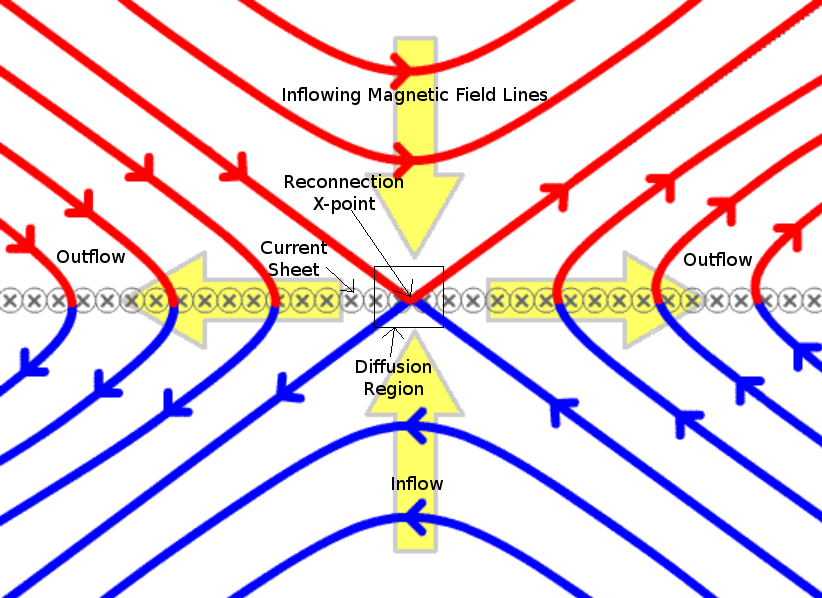
\includegraphics[width=0.40\textwidth]{2d-reconnection}
  \caption{A graphic representation of the 2D reconnection model. Inflowing magnetic field lines reconnect in the diffusion zone.}\label{2d-reconnection}
\end{center}
\end{figure}%\label{2d-reconnection}
At the moment of MR, the meeting of two anti-parallel magnetic field lines causes a magnetically neutral region of continuous change from negative to positive field. This condition is sustained by the conservation of the magnetic and plasma pressure contributions from the anti-parallel field lines on either side of the continuous neutral region. Inflowing magnetic field reconnects in the diffusion region with a configuration of increased magnetic tension or curvature, which drives post-reconnection outflow of the newly connected field, see figure \ref{2dreconnection}. Also, because the frozen-in condition is broken, plasma can move freely without the magnetic field and is ejected out along the neutral region.

%The Lorentz force generated by inflowing magnetic field lines has an associated electric field which induces high currents in the form of a current sheet in the diffusion region. ?????WHY IS THIS IMPORTANT???



\subsection{Eruptive Solar Flares}\label{flares}

Solar flares are the explosive conversion of magnetic energy into mass motions, radiation, electric currents and MHD waves. These events are the most energetic of solar phenomena and can be observed throughout the entire solar atmosphere, with some of the larger flares releasing up to $10^{37}$ erg of energy. Flares are classified by the the Geostationary Operational Environmental Satellite (GOES) see Table \ref{goes}, in this stem, the logarithmic measure of 1 to 8 \AA\ X-ray flux produced by the flare determines it's classification. The GOES system classes flares from X to A-class, in order of high to low flux, so an X-class flare event would be more powerful than an M-class and so on. \\

\begin{table}[h]
\centering
\begin{tabular}{|c|c|}\label{GOES}
Classification & Peak Flux Range at 1 to 8 \AA\ ($W.m^{-2}$) \\
\hline
X & $10^{-3}$ - $10^{-4}$\\
M & $10^{-4}$ - $10^{-5}$\\
C & $10^{-5}$ - $10^{-6}$\\
B & $10^{-6}$ - $10^{-7}$\\
A & $<10^{-7}$\\
\end{tabular}
\caption{shows the GOES flare classification, which is based on the order of magnitude of hard x-ray flux. X class flares produce a flux of $10^{-3}$ - $10^{-4}$ $W.m^{-2}$ and are the most powerful, whilst a weak A class flare can produce less than $10^{-7}$ $W.m^{-2}$.}\label{goes}
\end{table}

\subsubsection{Standard Eruptive Flare Model}
The standard solar flare theory, also known as the CSHKP model, is the culmination of research by many authors,\citep{1964NASSP..50..451C, 1966Natur.211..695S, 1974SoPh...34..323H, 1976SoPh...50...85K}, describing the formation and evolution of two-ribbon flares. 

\begin{figure}[H]
  \begin{center}
  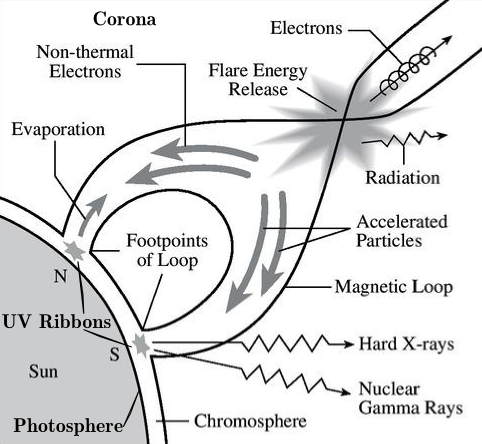
\includegraphics[width=0.40\textwidth]{flare}
  \caption{cartoon of the standard 2D solar flare model. Image courtesy of \href{http://ase.tufts.edu/cosmos/print_images.asp?id=47}{www.tufts.edu}}\label{flare-cartoon}
\end{center}
\end{figure}

In this model, magnetic free energy is stored high up in the corona, built up by a filament rising through the atmosphere. A filament is cool dense plasma suspended in the corona overlying an active region's polarity inversion line \citep{1955ApJ...121..349B}. It is thought that filaments are suspended up in the corona by magnetic fields in the form of either a sheared arcade or a flux rope which is the focus of the CSHKP model. As the filament (flux rope) rises, it drags the surrounding magnetic loops along with it, which creates a situation where the legs of the loops start to flow inward. As this inward flow causes opposing magnetic legs to get closer to each other, a current sheet develops which stretches along the neutral region. This current sheet eventually becomes thin enough that magnetic reconnection occurs, reconfiguring the magnetic field from inflowing legs to outflowing flare loop and filament structure. At this point energy is released in the form of heating, accelerated particles and MHD waves. Heating can reach temperatures of $10^7$ K and accelerated particles travel down flare loops causing emission, shocks and sometimes acoustic disturbances in the solar interior or sunquakes. The appearance of two flare ribbons is caused by reconnection occurring simultaneously across an arcade of magnetic loops. Accelerated particles travel down each loop in the arcade, colliding with the chromosphere as they do, at which point bremstrahlung and H$\alpha$ emission are produced, leading to the appearance of footpoints and ribbons respectively. A cascade of these reconnection events occur as the erupting filament rises through each successive loop making up the overlying non-potential magnetic field. When applied to the entire arcade of loops making up the field this leads to the appearance of flare ribbons moving outward from the polarity inversion line. If a filament is not present, \cite{2005psci.book.....A} describes the build up of magnetic free energy as being caused by the evolution of the associated active region, whereby photospheric plasma motions shear the magnetic field arcade causing reconnection. 


\subsubsection{Energy Transfer}
The impulsive phase of a solar flare occurs when energy near the reconnection X-point is transported along the magnetic field into the chromosphere. The two basic methods of energy transport during this phase are thermal and non-thermal. In the thermal case, plasma in the top of a flare loop is heated by MR or shocks. In the non-thermal case, particles are imparted enough energy to no longer be described by the thermal Maxwellian distribution, instead exhibiting nonthermal energies. The energy source for nonthermal particles is thought to be MR. During the impulsive phase of a flare, electrons are accelerated to high energies, down newly reconfigured flare loops. These high energy electrons are fed into the dense plasma of the chromosphere and photosphere where they deposit their energy. The collisional thick target model by \cite{1971SoPh...18..489B} says that almost all of the flare energy is carried by the particle beam, therefore, energy dissipated in the lower atmosphere represents a large portion of the flare energy budget.

\subsubsection{Thick Target Model} Assuming that the chromosphere is a thick target , the deposition of energy by accelerated particles is due to collisions between charged particles and ions producing hard X-ray bremsstrahlung emission \citep{1967SvA....11..258K}. Using the thick target model \citep{1971SoPh...18..489B} one can calculate the power, $P$, injected into the atmosphere by non-thermal electrons.  
 
\begin{equation}\label{pnth}
P(E \geq E_{c}) = \int_{E_{C}}^{\infty} EF(E)dE
\end{equation}

The electron distribution $F(E)$ is controlled by the power law $AE^{-\delta}$, where $E$ is the electron energy, $A$ is the total injected electron rate normalisation factor, $E_{C}$ is the low energy cut off and $\delta$ is the electron distribution spectral index. The value of $E_{C}$ represents the upper boundary between thermal and non-thermal energy contributions to the x-ray spectrum. This means that the total energy associated with non-thermal electron power is a lower limit. Performing the integral in equation \ref{pnth} gives the total non-thermal electron power in the form of equation \ref{pnth1}.

\begin{equation}\label{pnth1}
P(E \geq E_{c}) = \frac{AE_{C}^{(2-\delta)}}{(\delta - 2)}
\end{equation}

\subsubsection{Hydrodynamic Response}
During the impulsive phase of a solar flare, high energy nonthermal electrons are accelerated into the chromosphere. These particles transfer energy to the ambient chromospheric plasma in the form of heat. A consequence of this is the production of a hydrodynamic response in the from of coronal upflows and chromospheric downflows. The upflow is hot chromospheric plasma responding to an increase in temperature by expanding up into the flare loop coined as \emph{chromospheric evaporation}. Coronal upflows emit in soft x-rays. The downflow or \emph{chromospheric condensation} is formed when a steep temperature jump propagating into the chromosphere forms a downward moving shock front. The shock front contains dense, cool plasma which emits H$\alpha$ \citep{1981SoPh...73..269L, 1990ApJ...348..333C, 2015SoPh..tmp...61K}. 



\subsubsection{White Light Flares}
In 1859 the first white light flare (WLF) was observed by \cite{1859MNRAS..20...13C}. 
WLFs occur when energy is transported deep into the dense lower atmosphere causing a continuum enhancement in wavelengths with $\lambda > 3600$ Å \citep{1983SoPh...88..275N}. 
Once thought as rare, work by \cite{2003A&A...409.1107M} helped to show that WLFs are not only associated with the most energetic of solar flares but many of the smaller events as well. Since that first glimpse, the frequency of observations of WLFs have become common mainly due to ever increasing resolution of solar data. 


Theories that have been put forward to explain WLFs credit Balmer and Paschen continuum emission from free-bound transitions in hydrogen or H$^{-}$ processes \citep{1976GAM.....8.....S}. In fact the emission process producing the white light enhancement dictates where in the atmosphere the emission is coming from. If the WLF is due to hydrogen free-bound emission, this is caused by a temperature increase of $\sim10^{4}$ K in a plasma with a hydrogen number density of $n_{H}>10^{14}$ cm$^{-3}$ meaning WL must be coming from deep in the chromosphere. These conditions produce the opacity required to outshine the background photosphere emission. Whereas, if the WLF is due to H$^{-}$ processes the emission is coming from the photosphere where a modest temperature increase of $\sim10^{2}$ K and a hydrogen number density of $n_{H}>10^{16}$ cm$^{-3}$ are sufficient to satisfy opacity requirements. It is also possible that both WLF flare processes can occur simultaneously, so called radiative backwarming. Balmer/Paschen continua photons emitted in the chromosphere  irradiate the photosphere and are absorbed by H$^{-}$ ions which release emission causing the $10^{2}$ K temperature increase in the upper photosphere \citep{1989SoPh..124..303M}. It is also thought that it is possible to produce WLFs by heating of the upper photosphere by energetic electron beam \citep{1972SoPh...24..414H} and proton beam \citep{1978SoPh...58..363M}.  




%%%%%%%%%%%%%%%%%%%%%%%%%%%%%%%%%%%%%%%%%%%%%%%%%%%55
\subsection{Sunquakes}
A sunquake occurs when acoustic waves propagate into sub-surface layers of the Sun (see Figure \ref{sunquake-cartoon}a). As acoustic wave-fronts travel into the interior they encounter layers of increasing density causing refraction back toward the solar surface (see Figure \ref{sunquake-cartoon}b). At which point, waves can be observed as circular formations in the surface plasma, expanding outward from a point of origin (see Figure \ref{mdiquake96}) \citep{2014arXiv1402.1249K}. Expansion of sunquake ripples accelerates as the source of leading edge of the circular wave is coming from increasingly deep layers inside the Sun. This effect is caused by the increase in density with internal depth, which leads to a rise in sound speed \citep{1998Natur.393..317K}. It is not unreasonable to suspect that all solar flares produce some level of seismic signature but due to sunquake waves being hard to spot against photospheric background noise, only those with sufficient amplitude are detected. Sunquake morphology can sometimes be anisotropic in that some regions in a wavefront may have a variety of amplitudes, an attribute that is credited to sub-surface deviations in refraction. The anisotropy also extends to the formation of sunquake wavefronts that are not perfectly circular which is thought to happen as a result of moving impact sites \citep{2006ESASP.624E.134K}. 


\begin{figure}[hb]%\label{sunquake-cartoon}
  \begin{center}
  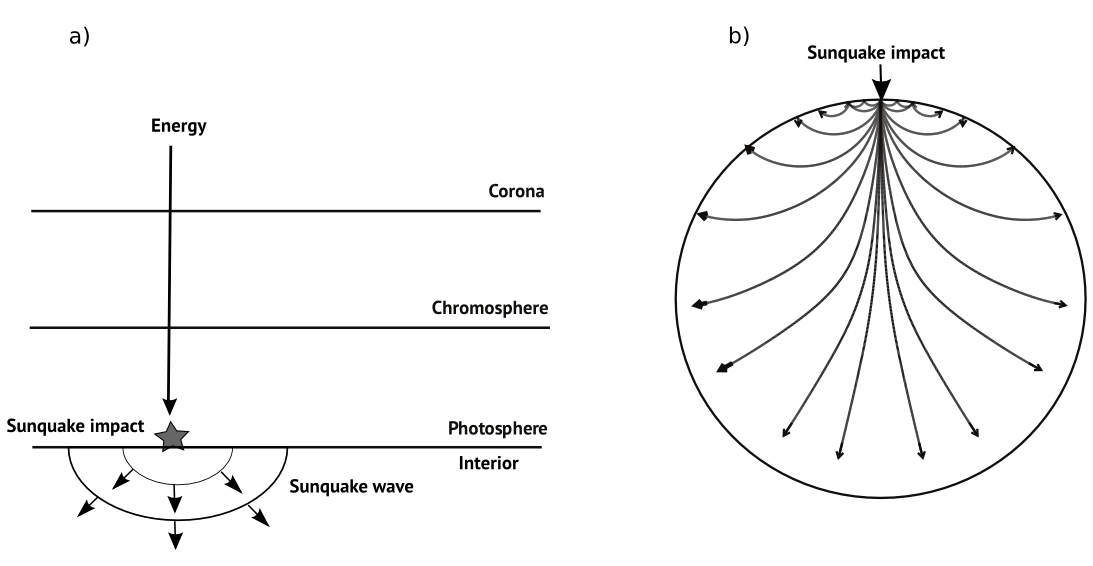
\includegraphics[width=0.99\textwidth]{sunquake-cartoon}
  \caption{Sunquake cartoon: a) Shows how energy and momentum must traverse through the solar atmosphere before impacting the photosphere to generate a sunquake. b) Shows acoustic wave-fronts propagating into the interior of the Sun. Wave-fronts refract back toward the surface as they encounter increasingly dense sub-surface layers. Waves reaching the surface disturb material in a pattern resembling ripples in a pond. Courtesy of \cite{2014arXiv1402.1249K}}\label{sunquake-cartoon}
\end{center}
\end{figure}


\subsubsection{Sunquake Generation}\label{sunprog}
%list and explain current theories of sunquake generation
%making sure to highlight the different observables that can identify each mechanism, eg wlf = evidence of radiative backwarming


The progenitors of sunquakes are still unknown and as a result this is an exciting area of research with discoveries still to be made. The general consensus, in terms of valid mechanisms that could cause this phenomenon is an area of contention, however the following progenitors are thought to be at least partly responsible. Each mechanism is associated with different observable signatures of which each observed sunquake may have some, none or many. This means that a rigid description of the transport of flare energy and momentum to the sub-photosphere is probably unlikely. Instead each candidate progenitor may play a bit part in the process, and there very well maybe mechanisms yet undiscovered. \\

\begin{itemize}
\item \textbf{Radiative backwarming} as a mechanism for producing sunquakes, was first put forward by \cite{2005ApJ...630.1168D} to account for a spatial correlation between seismic sources and white light emission from the lower atmosphere. During a solar flare, high energy electrons and photons impulsively heat the chromosphere and photosphere leading to an enhancement in white light emission \citep{1989SoPh..124..303M}. This WL enhancement can be generated by either; Balmer continuum generated by hydrogen bound-free emission in the upper-chromosphere, which irradiates the photosphere increasing local plasma temperature; $H^{-}$ emission at deeper altitudes, near the temperature minimum region. In both cases, an impulsive increase in radiation pressure and gas pressure exerted on the photosphere could generate acoustic waves which propagate into the sub-photosphere. Therefore a clear radiative energy contribution from Balmer continuum and general white light emission are considered signatures of radiative backwarming. For backwarming to be responsible for the sunquake, a comparable radiative energy budget in a Balmer or white-light signature would be required.\\

\item \textbf{Sudden magnetic field reconfiguration} was first detailed by \cite{2008ASPC..383..221H}. Solar flares are violent physical processes dictated by the interplay between reconnecting magnetic fields and charged solar plasma.
If the magnetic field close to the photosphere relaxes to a more horizontal alignment it can impart a Lorentz force on the local plasma environment, resulting in the production of acoustic waves in the sub-photosphere. The key parameter for this mechanism seems to be that the field has to reconfigure in an sufficiently impulsive manner to generate enough force to induce seismic waves. An observable signature of this progenitor would be impulsive changes in magnetic field strength close to the sunquake. \\

\item \textbf{Shocks} are a mechanism originally proposed in initial work by \cite{1995ESASP.376b.341K} and \cite{1998Natur.393..317K}, whereby a shock wave propagates from the upper-chromosphere down to lower altitudes. During a solar flare, particles and heat are directed down toward the chromosphere, at which point chromospheric material reacts by increasing in temperature. This increased temperature causes explosive ablation of chromospheric material both upward and downward. The downward component develops into a shock front carrying energy to the lower atmosphere, which can go on to impact the photosphere generating acoustic waves. If the shock is dissipated at higher altitudes such as the lower chromosphere, heat generated during the deposition process can irradiate the photosphere with high energy photons, causing radiative backwarming \citep{1989SoPh..124..303M}. If the sunquake is caused by a shock then acoustic impacts should occur approximately 100 seconds after the HXR signature associated with the flare impulsive phase, as dictated by the thick target model. Observational signatures of shocks are red or blue shifted wavelengths which can be captured in Dopplergrams or spectroscopic data. \\

\item \textbf{Direct proton collision}, is linked to observations by \cite{2007ApJ...664..573Z} where the sunquake was spatially aligned with $\gamma$-ray emission. $\gamma$-rays during a solar flare are an indicator of energetic protons being accelerated along a newly reconfigured magnetic field. Proton beams carry more momentum than electron beams and are able to penetrate through the solar atmosphere to lower altitudes. If an energetic beam of protons makes it down to the photosphere, it can deposit energy in the form of an impact, which due to conservation of momentum could generate acoustic waves in the sub-photosphere. $\gamma$-ray data is captured by RHESSI. \\

\end{itemize}
%It is also theoretically possible to heat the upper photosphere by resistive dissipation of Alfven waves \citep{1982SoPh...80...99E}


\subsubsection{Local Helioseismology}
%use content from old report...maybe expand a little
Helioseismology is a tool for probing the interior of the Sun. Most techniques in this field of analysis rely on observations of gravity and acoustic waves on the photosphere that are the result of interior excitation. Studying the frequency and modes of these oscillations has revealed much about the internal structure of the Sun. Local helioseismology is a collection of techniques developed for global helioseismology that have been modified for use in studying local regions in higher spatial resolution. The following section provides an introduction to some of these techniques.

\paragraph{Theoretical Helioseismic Response}\label{helioresp}
The localised helioseismic response to an impact that generates a sunquake can be calculated. If the surface impact occurs in a small volume, the radial component of the resulting helioseismic velocity, $v_r$ can be calculated with:
%\sum_{n=1}^{\infty} 2^{-n} = 1
\begin{equation}
v_{r}(R, \theta, \phi, t) = \sum_{nlm} \frac{P_{0}}{M_{\odot}I_{nl}}(2l+1)P_{l}(\cos\theta)\cos(\omega_{nl}t)e^{-\gamma_{nl}t}
\end{equation}

The total momentum transferred by the impact is $P_{0}$, $M_{\odot}$ is solar mass, $I_{nl}$ is the mode inertia, $P_{l}$ is the Legendre polynomial, $\omega_{nl}$ are the mode eigenfrequencies, $\gamma_{nl}$ are their damping times and $(2l+1)$ is a geometric factor. The collective terms $M_{\odot}I_{nl}$ are known as the \emph{mode mass} meaning that the mode amplitude driven by the impact is proportional to the total momentum over the mode mass.    

\begin{equation}
v_{r}(R, \theta, \phi, t) \propto \sum_{nlm} \frac{P_{0}}{M_{\odot}I_{nl}}
\end{equation}

A total momentum of $10^{24}$ g.cm/s was calculated by \cite{2009AIPC.1170..547K} as the momentum associated with the maximum observed amplitude in a sunquake. Using this technique, it is possible to extract the frequency at which wave amplitude is at a maximum, which turns out to be in the 4 to 5 mHz range.

\paragraph{Helioseismic Holography}\label{helioholog}
\cite{1999ApJ...513L.143D} pioneered the use of helioseismic holography to produce seismic images of the solar flare of July 1996 reported to have a sunquake by Kosovichev and Zharkova. Time series egression-power maps at 3.5 and 6 mHz were computed with a 2 mHz bandwidth. It was found that the most powerful acoustic power frequency associated with the flare is centred at 3.5 mHz but has a large amount of noise. However, the 6 mHz range has a much lower ambient noise, therefore producing a better rendering of the seismicity of the flare. It is now standard practice to use the 6 mHz range for helioseismic holographic calculations of egression-power. \\
Originally the idea of analysing Doppler images of the solar surface in order to observe acoustic sources was put forward by \cite{1975CRASB.281...93R}. Helioseismic holography was developed further in concept by Lindsey and Braun \citep{1990SoPh..126..101L, 1992ApJ...392..739B, 1997ApJ...485..895L} in an effort to to image the solar interior and far-side of the Sun. This technique involves using a Doppler image of a location on the solar surface as a reference wave-field to enable an estimation of that wave-field at a location in the solar interior at a time preceding or proceeding the image. This is achieved by calculating the ingression or egression of the wave-field by assuming that it's evolution is a, convergence to, or divergence from, the point of origin of that wave-field. The technique uses Green's function (eqn \ref{green}, where $\vec{r}$ and $t$ are position and time of an observed signal and $\vec{r}'$ and $t$' are the position and time of the signal earlier in time) which assumes that the acoustic wave propagates from a point source, allowing a signal $\psi(\vec{r},t)$ observed on the surface to be devolved backwards in time.

\begin{equation}\label{green}
G_{+}(|\vec{r}-\vec{r}'|,t-t')
\end{equation}

Where $a$ and $b$ constrain the holographic pupil, equation \ref{holog} is then used to devolve the surface signal to calculate the position of subsurface acoustic sources.

\begin{equation}\label{holog}
H_{+}(\vec{r},z,t)= \int dt'  \int_{a<|\vec{r}-\vec{r}'|<b} d^{2}\vec{r}'G_{+}(|\vec{r}-\vec{r}'|,t-t')\psi(\vec{r}',t')
\end{equation}

Equation \ref{eggpower} is then used to calculate the egression power associated with the acoustic sources at a time $t$.

\begin{equation}\label{eggpower}
P(z,\vec{r})=\int dt|H_{+}(\vec{r},z,t)|^{2}dt
\end{equation}

If egression power is required in terms of frequency then equation \ref{eggpower} can be Fourier transformed into frequency space.


\paragraph{Time-Distance}\label{TD}
The first observation of a sunquake \citep{1998Natur.393..317K} used the time-distance technique to track sunquake wavefronts. The paper by \cite{1993Natur.362..430D} explains how to extract time-distance (TD) information from observations of intensity fluctuations on the solar surface. This technique uses travel times of waves between two locations on the solar surface. The method assumes that the travel time of a wave propagating in the interior of the Sun will be modified by any anomalies that it has to travel through, thus the resulting signal will contain the signatures of those irregularities. For instance, if the wave encounters a flow along it's path of travel, it will propagate faster with the flow than against it, affecting travel time.
This technique remaps Dopplergrams into polar coordinates, with the point of origin centred on the area of downflowing material during the flare. This remapped image is then Fourier transformed with respect to azimuthal angle, with the resulting image highlighting circular disturbances as a line of positive slope.
